\chapter{Objective specification and presentation of the research methodology}

Having laid the groundwork with essential concepts necessary for this thesis,
this chapter aims to outline the objectives of the practical segment as well as the research methodology employed to achieve them.
In the first part, the specific objectives are defined. 
Afterwards, in a second part the used reasearch framework \ac{DSR} and the two research methods Prototyping and the Simulation are explained.

\section{Objective specification}

In contrast to the mentioned papers in 2.4.4, this thesis wants to use their proof of concepts as a basis and go further to see if the concept
is feasible on the complete \ac{ASIC} hardware accelerator like the \ac{mem-HNN} and does it bring an actual acceleration.
The practical part is therefore using a current \ac{ASIC} with not only the memristor crossbar array but also all the other requried hardware components.
Furthermore, the thesis focuses on an actual training of a \ac{RBM} and also the interference of it to be able to answer the research question.
Expanding upon the foundational work, this research explores the implementation of the N/2 synchronous update mechanism.
This design choice emphasizes a expactation of higher sampling speeds and efficiency.

At the beginning, the \ac{IT}-artifact to be implemented is modeled and all components, transitions and processes of the overall solution are identified.
As a result of the implementation a complete performance evaluation, including a comprehensive energy model and a latency model should be established.
This evaluation aims to measure the metrics: required processing time (samples/sec) for data and the energy usage (energy/operation).
The results should be compared to other sampling methods, such as Gibbs and Metropolis sampling.
Lastly, this thesis performs hyperparameter tuning in oder to gather new data on how these machines should be configured for optimal performance.
Since, there is no data for hyperparameter tuning of such a concept in the literature yet this establishes foundational work on how to make use of artificial intelligence within such an accelerator.
Through this process, the research seeks to determine the feasibility of a proper training with this setup, focusing on its practicality and efficiency.
By benchmarking these aspects against traditional sampling methods, the thesis aims to underscore the potential of the \ac{mem-HNN} 
in practical training of \ac{RBM}s.

Hence, \ac{DSR} is used as a research framework to iteratively create the \ac{IT}-artifact. 
In addition to that, within the single iterations prototyping is used for the actual implementation of the \ac{RBM} on the simulated \ac{mem-HNN} with individual goals.
The last iteration uses a simulation as research method because there the behaviour and performance of the system is meassured and the underlying model already finisehd with the last prototyping iteration. 
Since, the practical functionality can't be ensured the \ac{DSR} process combined with prototyping and if successful a simulation 
brings flexibility and a problem-oriented structure which are emphasized for this new method. 

\section{Design Science Research}

In terms of information systems \ac{DSR} is a core research method within the field of business informatics that ``creates and evaluates \ac{IT}-artifacts intended to solve identified organizational problems''\footcite[77]{hevnerDesignScienceInformation2004a}
Henver et al. established a DSR framework that has the goal of creating an \ac{IT}-artifact which has the purpose of addressing and solving the important organizational problem.\footcite[82]{hevnerDesignScienceInformation2004a}
This systematic \ac{DSR} process lays a solid groundwork for conducting the research with rigor, offering a degree of confidence that the endeavor will yield meaningful outcomes.\footcite[cf.][368]{baskervilleDesignScienceResearch2018}
Artifacts in \ac{DSR} can be constructs, models, methods or instantiations.\footcite[77]{hevnerDesignScienceInformation2004a}
In addition to that, Gregor and Hevner (2013) categorize the underlying \ac{IT}-artifact based on their abstraction level and maturities.
Hence, level 1 represents a specific, limited and less mature implementation of an artifact, level 2 are operational principles or architecture like constructs, methods or models, while level 3 represents a well-developed midrange design theory.\footcite[cf.][342]{gregorPositioningPresentingDesign2013}
The development of the artifact is performed incrementally with specific goals for each iteration, which is beneficial for \ac{IT}-artifacts that can be adjusted after every iteration.\footcite[cf.][343]{gregorPositioningPresentingDesign2013}

Henver et al. also introduced 7 guidelines that still today serve as framework for different \ac{DSR} approaches.
Arguably, the most important two guidelines are, that the research must create a viable artifact that in a next step is able to solves the organizational problem. 
Another important guideline is that the artifact needs to be rigorously evaluated in utility, quality and efficiency.\footcite[83]{hevnerDesignScienceInformation2004a}
Thereupon Peffer et al. introduced a well-known \ac{DSR} Process Model, which has 6 different phases: Identify problem \& Motivate, Define Objectives of a solution, 
Design \& Development, Demonstration, Evaluation and Communication.\footcite[cf.][54]{peffersDesignScienceResearch2007a}
Another interesting approach by Österle et. al, which is called design-oriented business informatics. 
This \ac{DSR} method is used in this thesis for following reasons.
His approach compresses the phases of Peffer et al. into a more compact model and also gives a more detailed explanation of each phase while still complying with the guidelines established by Henver et la..\footcite[cf.][1-6]{oesterleMemorandumZurGestaltungsorientierten2010}
On top of this promising framework they created a \ac{DSR} model called consortial research.
It addresses problems for collaborative research in terms of access to practical knowledge, rapid change and practical orientation and a lack of support for knowledge transfer.\footcite[cf.][273-274]{oesterleKonsortialforschung2010}
Österle et al. aim to bridge the gap between the knowledge base of both science and practice, with a focus on evaluating and ensuring the reproducibility of research outcomes.\footcite[cf.][5]{oesterleMemorandumZurGestaltungsorientierten2010}
However, the individual phases of the research framework can also be implemented on their own and the best features 
of the research framework and especially the contents of the phases should be combined with its old framework of design-oriented business informatics.
As a result following model showed in figure XXX is used:
\begin{figure}[H]
    \centering
    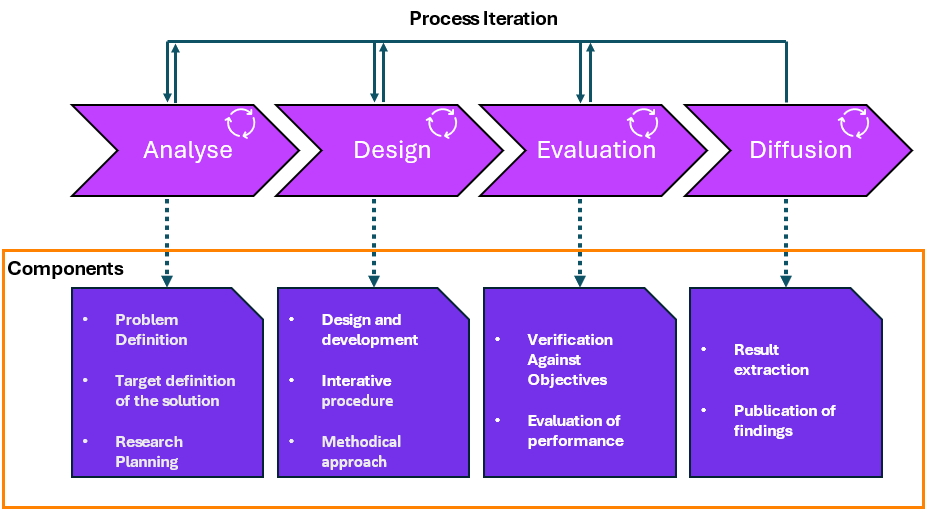
\includegraphics[width=1\linewidth]{graphics/DSR_Modell.png}
    \caption{\ac{DSR} model of this thesis\protect\footnotemark}
    \label{DSR_Modell}
\end{figure}
\footnotetext{inspired from \cite[cf.][3]{gmComprehensiveSurveyAnalysis2020}}


\section{Prototyping / Simulation}

